\documentclass[../main.tex]{subfiles}

\begin{document}

\chapquote{Chess is the struggle against the error.}{Johannes Zukertort}
\chapter{Evaluation}
\label{chap:evaluation}
In \cref{chap:chess_recognition}, we evaluated the performance of each component in the chess recognition pipeline separately as well as the system as a whole, but that analysis was limited to the training and validation sets.
The test set remained untouched thus far for reasons concerning data leakage outlined in \cref{sec:split_dataset}.
Now we can evaluate the chess recognition system on the held-out test set because we have ensured that the models never before encountered this data.
\Cref{tbl:chess_recognition_trainvaltest_results} lists key evaluation metrics for the test set and contains the corresponding numbers from the other two datasets (as in \cref{tbl:chess_recognition_trainval_results}) for comparison.
\begin{table}
    \makebox[\textwidth][c]{
        \begin{tabular}{lrrr}
            \toprule
            metric & train & val & test \\
            \midrule
            mean number of incorrect squares per board           & 0.27    & 0.27     & 0.24 \\
            percentage of boards predicted with no mistakes      & 94.77\% & 97.95\%  & 93.86\% \\
            percentage of boards predicted with $\leq 1$ mistake & 99.14\% & 99.32\%  & 99.42\% \\
            per-board corner detection accuracy                  & 99.59\% & 100.00\% & 99.42\% \\
            per-square occupancy classification accuracy         & 99.81\% & 99.97\%  & 99.92\% \\
            per-square piece classification accuracy             & 99.99\% & 99.99\%  & 99.99\% \\
            \bottomrule
        \end{tabular}
    }
    \caption[Performance of the chess recognition system on the test dataset.]{Performance of the chess recognition system on the test dataset. The training and validation metrics as per \cref{tbl:chess_recognition_trainval_results} are included for comparison.}
    \label{tbl:chess_recognition_trainvaltest_results}
\end{table}
There is no indication of overfitting because there are only slight differences in the results of the train and test sets.
The end-to-end per-board accuracy of our system on the unseen test set is 93.86\%, and if we allow just one mistake on the board, that accuracy increases to 99.42\%.
Comparing the overall accuracy to the training set, we see a decrease in almost one percentage point. 
It appears that the reason for the slightly worse performance on the test set is the marginally lower accuracy of the board localisation algorithm (99.59\% on the training set vs. 99.42\% on the test set).
The two \glspl{cnn} actually perform on par or even better on the test set than the training set.

The empirical results on the test set clearly demonstrate that the chess recognition system is highly accurate.
However, for such a system to be practically effective, it must also be able to perform an inference in a reasonable amount of time.
To test this, we record the inference time for each of the test set samples and compute the mean over all samples.
In fact, we can provide more granular insights by additionally recording the average time in executing each of the three stages in the pipeline.
We conduct this experiment twice on the dedicated lab machine: in the first trial, we use only the \gls{cpu} whereas we enable \gls{gpu} acceleration for the second run.
The machine is equipped with a quad-core 3.20GHz Intel Core i5-6500 \gls{cpu} and, as mentioned in \cref{chap:implementation}, a 6GB NVIDIA GeForce GTX 1060 \gls{gpu}.
\Cref{fig:chesscog_speed} shows that the system is around six times faster when utilising the \gls{gpu}.
\begin{figure}
    \centering
    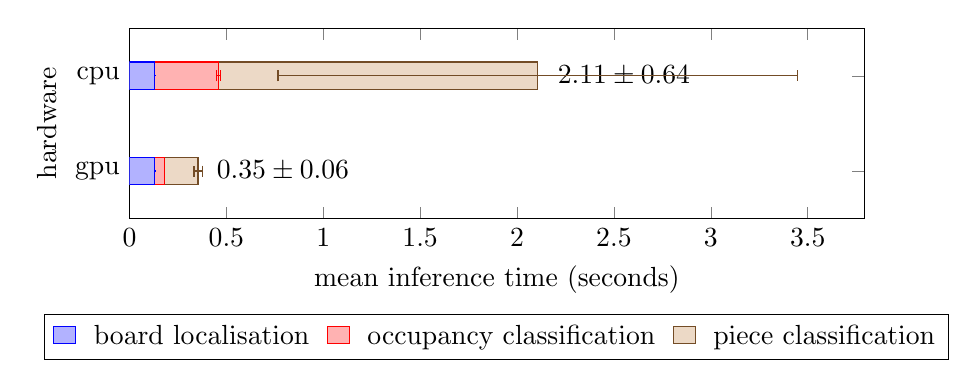
\begin{tikzpicture}
        \begin{axis}[
            width=.9\textwidth,
            height=4cm,
            xbar stacked,
            ylabel=hardware,
            xlabel=mean inference time (seconds),
            xmin=0,
            scaled ticks=false,
            stackedbar/.style = {
                xbar,
                error bars/.cd,
                x dir=both,
                x explicit relative
            },
            ytick={0,1},
            yticklabels={\acs{gpu},\acs{cpu}},
            % nodes near coords,
            y tick label style={align=center},
            enlarge y limits={abs=.5},
            legend columns=3,
            legend style={
                at={(0.5,-0.5)},
                anchor=north,
                column sep=1ex
            }
        ]
            \addplot+ [stackedbar] coordinates {
                (0.12935891456299406,0) +- (0.0069065603270334080,0)
                (0.12931111829404520,1) +- (0.0068571181376688630,0)
            };
            \addplot+ [stackedbar] coordinates {
                (0.05043862565584919,0) +- (0.0015867081771973946,0)
                (0.33029624063499774,1) +- (0.0219789229658819900,0)
            };
            \addplot+ [stackedbar] coordinates {
                (0.17394946628414532,0) +- (0.0593067253642730050,0)
                (1.64710188215145100,1) +- (0.6361857413955617000,0)
            };
            \node at (0.40, 0) [right] {$0.35 \pm 0.06$};
            \node at (2.16, 1) [right] {$2.11 \pm 0.64$};
            \legend{board localisation,occupancy classification,piece classification}
        \end{axis}
    \end{tikzpicture}
    \caption[Inference time benchmarks of the chess recognition pipeline on the test set.]{Inference time benchmarks of the chess recognition pipeline on the test set, averaged per sample. The error bars indicate the standard deviation and the mean total inference time is on the right of the bars. All benchmarks were carried out on the same machine (the Ubuntu lab machine described in \cref{chap:implementation}), although the data for the trial labelled \acs{cpu} was gathered without \acs{gpu} acceleration.}
    \label{fig:chesscog_speed}
\end{figure}
This is to be expected because the forward pass through the neural network executes many matrix operations that follow the \gls{simd} pattern and are thus well-suited for parallel computation on a \gls{gpu}.
Therefore, execution time of the occupancy and piece classifiers is significantly lower on the \gls{gpu}, whereas the board localisation (which runs on the \gls{cpu} regardless) takes a similar amount of time across both trials. 
Overall, the mean inference time is less than half a second on the \gls{gpu} and just over two seconds on the \gls{cpu}, although the latter measurement exhibits a significantly greater variance.
We conclude that the speed is sufficient for the intended practical purpose, and that the \gls{gpu}-accelerated pipeline would even be suited for real-time inference at 2-3 frames per second on just one \gls{gpu}.
Lastly, we see that the occupancy classifier needs just a fraction of the time required by the piece classifier.
This can be explained in the more complex architecture of the InceptionV3 network as opposed to the ResNet model and the greater input size which results in the number of parameter being twice as high in the piece classifier.

\section{Achievement of objectives}
All initial objectives described in the \gls{doer} document as well as the additional tertiary objective introduced in \cref{sec:objectives} have been successfully achieved in this project.
The following paragraphs provide evidence for the achievement of each objective in the order that they were specified in \cref{sec:objectives}.

\paragraph{Primary objectives}
The context survey of chess recognition systems in \cref{sec:context_survey_chess_recognition} is the outcome of objective \ref{obj:11} and is used to identify the limitations of current chess recognition systems to improve on them.
Next, the corner detection algorithm for localising chessboards (objective \ref{obj:12}) as detailed in \cref{sec:board_localisation} achieves an accuracy of 99.42\%, clearly highlighting its robustness.
Objective \ref{obj:13} concerns itself with the development of an algorithm for recognising chess pieces.
This is achieved in a two-stage process of occupancy classification (\cref{sec:occupancy_classification}) followed by piece classification (\cref{sec:piece_classification}) using \glspl{cnn}.
As a result, \cref{sec:preparing_results} explains how the entire pipeline is assembled, as required by objective \ref{obj:14}.
In accordance with the last primary objective \ref{obj:15}, the developed algorithms are each evaluated in isolation in \cref{chap:chess_recognition}, and then as a whole (\cref{sec:preparing_results} evaluates it on the validation set and at the beginning of this chapter, this is compared to the test set performance).

\paragraph{Secondary objectives}
\Cref{chap:data_synthesis} details the process of data synthesis, where the process of generating a large dataset of 4,800 labelled samples was automated using a 3D model in Blender, thus achieving objective \ref{obj:21}.
In line with objective \ref{obj:22}, \cref{sec:preparing_results} explains how the probability distribution over the squares is utilised to assemble an internal representation of the chess position which is then converted to \gls{fen} format.
The web \gls{api} for executing the inference pipeline as required by objective \ref{obj:23} is explained in \cref{sec:implementation_chessogapp} and available online at \url{https://www.chesscog.com/api/docs}.

\paragraph{Tertiary objectives}
Evidence for fulfilling objective \ref{obj:31} (implementing a proof-of-concept web app for chess position inference) lies in the fact that it is hosted online at \url{https://www.chesscog.com} and is explained in \cref{sec:implementation_chesscogapp,fig:webapp_overview}.
The \gls{fen} string is used to provide a link for opening the position in the board analysis tool on the popular chess website Lichess upon performing an inference.
Finally, the achievement of objective \ref{obj:32} is highlighted in \cref{chap:adapting}, where a process is devised for adapting the chess recognition system to new chess sets, using only two pictures of the board for training.
The success of this approach is reflected by the impressive results in \cref{tbl:transfer_learning_results}: based on just these two images, the system was able to correctly identify 88.89\% of the positions in the held-out test set, and all other positions had just one mistake.

Although not a formal objective, a deliberate emphasis was put on ensuring that the results claimed in this report are reproducible which even led to publishing a Python package (\texttt{recap}) on \gls{pypi} as a byproduct.
The datasets and trained models are made available for download, and all necessary code for training, inference, and evaluation is published on GitHub and supplied alongside the project submission.

\section{Critical appraisal}

% \ifSubfilesClassLoaded{%
% \printglossary[type=\acronymtype]%
% \printbibliography%
% }{}%

\end{document}